\documentclass[12pt]{article}

%%%%%%%%%%%%%%%%%%%%%%%%%%%%%%%%%%%%%%%%%%%%%%%%%%%%%%%%%%%%%%%%%%%%%%%%%%%%%%%%
%                           Package preset for homework
%%%%%%%%%%%%%%%%%%%%%%%%%%%%%%%%%%%%%%%%%%%%%%%%%%%%%%%%%%%%%%%%%%%%%%%%%%%%%%%%
% Miscellaneous
\usepackage[margin=1in]{geometry}
\usepackage[utf8]{inputenc}
\usepackage{indentfirst}
\usepackage{blindtext}
\usepackage{graphicx}
\usepackage{xr-hyper}
\usepackage{hyperref}
\usepackage{enumitem}
\usepackage{color}
\usepackage{float}
% Math
\usepackage{latexsym}
\usepackage{amsfonts}
\usepackage{amssymb}
\usepackage{amsmath}
\usepackage{commath}
\usepackage{amsthm}
\usepackage{bbold}
\usepackage{bm}
% Physics
\usepackage{physics}
\usepackage{siunitx}
% Code typesetting
\usepackage{listings}
% Citation
\usepackage[authoryear]{natbib}
\usepackage{appendix}
\usepackage[capitalize]{cleveref}
% Title & name
\title{Homework}
\author{Tien Vo}
\date{\today}


%%%%%%%%%%%%%%%%%%%%%%%%%%%%%%%%%%%%%%%%%%%%%%%%%%%%%%%%%%%%%%%%%%%%%%%%%%%%%%%%
%                   User-defined commands and environments
%%%%%%%%%%%%%%%%%%%%%%%%%%%%%%%%%%%%%%%%%%%%%%%%%%%%%%%%%%%%%%%%%%%%%%%%%%%%%%%%
%%% Misc
\sisetup{load-configurations=abbreviations}
\newcommand{\due}[1]{\date{Due: #1}}
\newcommand{\hint}{\textit{Hint}}
\let\oldt\t
\renewcommand{\t}[1]{\text{#1}}

%%% Bold sets & abbrv
\newcommand{\N}{\mathbb{N}}
\newcommand{\Z}{\mathbb{Z}}
\newcommand{\R}{\mathbb{R}}
\newcommand{\Q}{\mathbb{Q}}
\let\oldP\P
\renewcommand{\P}{\mathbb{P}}
\newcommand{\LL}{\mathcal{L}}
\newcommand{\FF}{\mathcal{F}}
\newcommand{\HH}{\mathcal{H}}
\newcommand{\NN}{\mathcal{N}}
\newcommand{\ZZ}{\mathcal{Z}}
\newcommand{\RN}[1]{\textup{\uppercase\expandafter{\romannumeral#1}}}
\newcommand{\ua}{\uparrow}
\newcommand{\da}{\downarrow}

%%% Unit vectors
\newcommand{\xhat}{\vb{\hat{x}}}
\newcommand{\yhat}{\vb{\hat{y}}}
\newcommand{\zhat}{\vb{\hat{z}}}
\newcommand{\nhat}{\vb{\hat{n}}}
\newcommand{\rhat}{\vb{\hat{r}}}
\newcommand{\phihat}{\bm{\hat{\phi}}}
\newcommand{\thetahat}{\bm{\hat{\theta}}}

%%% Other math stuff
\providecommand{\units}[1]{\,\ensuremath{\mathrm{#1}}\xspace}
% Set new style for problem
\newtheoremstyle{problemstyle}  % <name>
        {10pt}                   % <space above>
        {10pt}                   % <space below>
        {\normalfont}           % <body font>
        {}                      % <indent amount}
        {\bfseries\itshape}     % <theorem head font>
        {\normalfont\bfseries:} % <punctuation after theorem head>
        {.5em}                  % <space after theorem head>
        {}                      % <theorem head spec (can be left empty, 
                                % meaning `normal')>

% Set problem environment
\theoremstyle{problemstyle}
\newtheorem{problemenv}{Problem}[section]
\newenvironment{problem}[1]{%
  \renewcommand\theproblemenv{#1}%
  \problemenv
}{\endproblemenv}
% Set lemma environment
\newenvironment{lemma}[2][Lemma]{\begin{trivlist}
\item[\hskip \labelsep {\bfseries #1}\hskip \labelsep {\bfseries #2.}]}{\end{trivlist}}
% Set solution environment
\newenvironment{solution}{
    \begin{proof}[Solution]$ $\par\nobreak\ignorespaces
}{\end{proof}}
\numberwithin{equation}{problemenv}

%%% Page format
\setlength{\parindent}{0.5cm}
\setlength{\oddsidemargin}{0in}
\setlength{\textwidth}{6.5in}
\setlength{\textheight}{8.8in}
\setlength{\topmargin}{0in}
\setlength{\headheight}{18pt}

%%% Code environments
\definecolor{dkgreen}{rgb}{0,0.6,0}
\definecolor{gray}{rgb}{0.5,0.5,0.5}
\definecolor{mauve}{rgb}{0.58,0,0.82}
\lstset{frame=tb,
  language=Python,
  aboveskip=3mm,
  belowskip=3mm,
  showstringspaces=false,
  columns=flexible,
  basicstyle={\small\ttfamily},
  numbers=none,
  numberstyle=\tiny\color{gray},
  keywordstyle=\color{blue},
  commentstyle=\color{dkgreen},
  stringstyle=\color{mauve},
  breaklines=true,
  breakatwhitespace=true,
  tabsize=4
}
\lstset{
  language=Mathematica,
  numbers=left,
  numberstyle=\tiny\color{gray},
  numbersep=5pt,
  breaklines=true,
  captionpos={t},
  frame={lines},
  rulecolor=\color{black},
  framerule=0.5pt,
  columns=flexible,
  tabsize=2
}


\title{Homework 11: Phys 7320 (Spring 2022)}
\due{April 13th, 2022}

\begin{document}
\maketitle
%%%%%%%%%%%%%%%%%%%%%%%%%%%%%%%%%%%%%%%%%%%%%%%%%%%%%%%%%%%%%%%%%%%%%%%%%%%%%%%
\begin{problem}{1}[Power distributions for simple motion]
Using the Liénard-Wiechert fields, discuss the time-averaged power radiated per
unit solid angle in nonrelativistic motion of a particle with charge $e$, moving

(a) along the $z$ axis with instantaneous position $z(t)=d\cos\omega_0t$. Show
how the time-averaged $dP/d\Omega$ and $P$ match to results from earlier in the
semester using the dipole moment,

(b) in a circle of radius $R$ in the $xy$ plane with constant angular frequency
$\omega_0$. Express $\Theta$ (the angle between the acceleration and the
observation point) as a function of time and the spherical coordinates of the
observer. For this part the time-averaged $P$ should match results from earlier
in the semester with the dipole moment. (The angular distribution in
$dP/d\Omega$ is different from what you're used to; this is because the dipole
is not pointing in the $z$-direction, but instead rotating in the $xy$-plane,
and consequently the configuration corresponds to spherical harmonics with
$l=1,m=\pm1$ instead of $l=1,m=0$; see table 9.1 in Jackson section 9.9.)

Sketch the angular distribution of the radiation and determine the total power
radiated in each case. Also calculate the dipole moment as a function of time,
and cast it as a complex moment $\vb{p}$ using the usual form
$\vb{p}_\t{real}=\Re\qty(\vb{p}e^{-i\omega t})$.
\begin{solution}
(a) Given the position, we can calculate the instantaneous acceleration
\begin{equation}
    a=\frac{d^2z}{dt^2}=-\omega_0^2z=-\omega_0^2d\cos\omega_0t. 
\end{equation}
Then, from (14.21, Jackson), the radiation pattern is
\begin{equation}
    \frac{dP}{d\Omega}=\frac{e^2}{4\pi c^3}a^2\sin^2\Theta
    =\frac{e^2\omega_0^4d^2}{4\pi c^3}\sin^2\Theta\cos^2(\omega_0t).
\end{equation}
Averaged over time, this gives
\begin{equation}
    \expval{\frac{dP}{d\Omega}}
    =\frac{e^2\omega_0^4d^2}{8\pi c^3}\sin^2\Theta
    =\frac{c}{8\pi}\frac{\omega_0^4}{c^4}(ed)^2\sin^2\Theta.
\end{equation}
This is the same form as (9.23, Jackson) in Gaussian units. In analogy, the
oscillating charge forms a dipole $\vb{p}=ede^{-i\omega t}\zhat$ when averaged 
over time. The wavenumber is given by the frequency of oscillation
$k=\omega_0/c$. A plot of $dP/d\Omega$ is given below
\begin{center}
    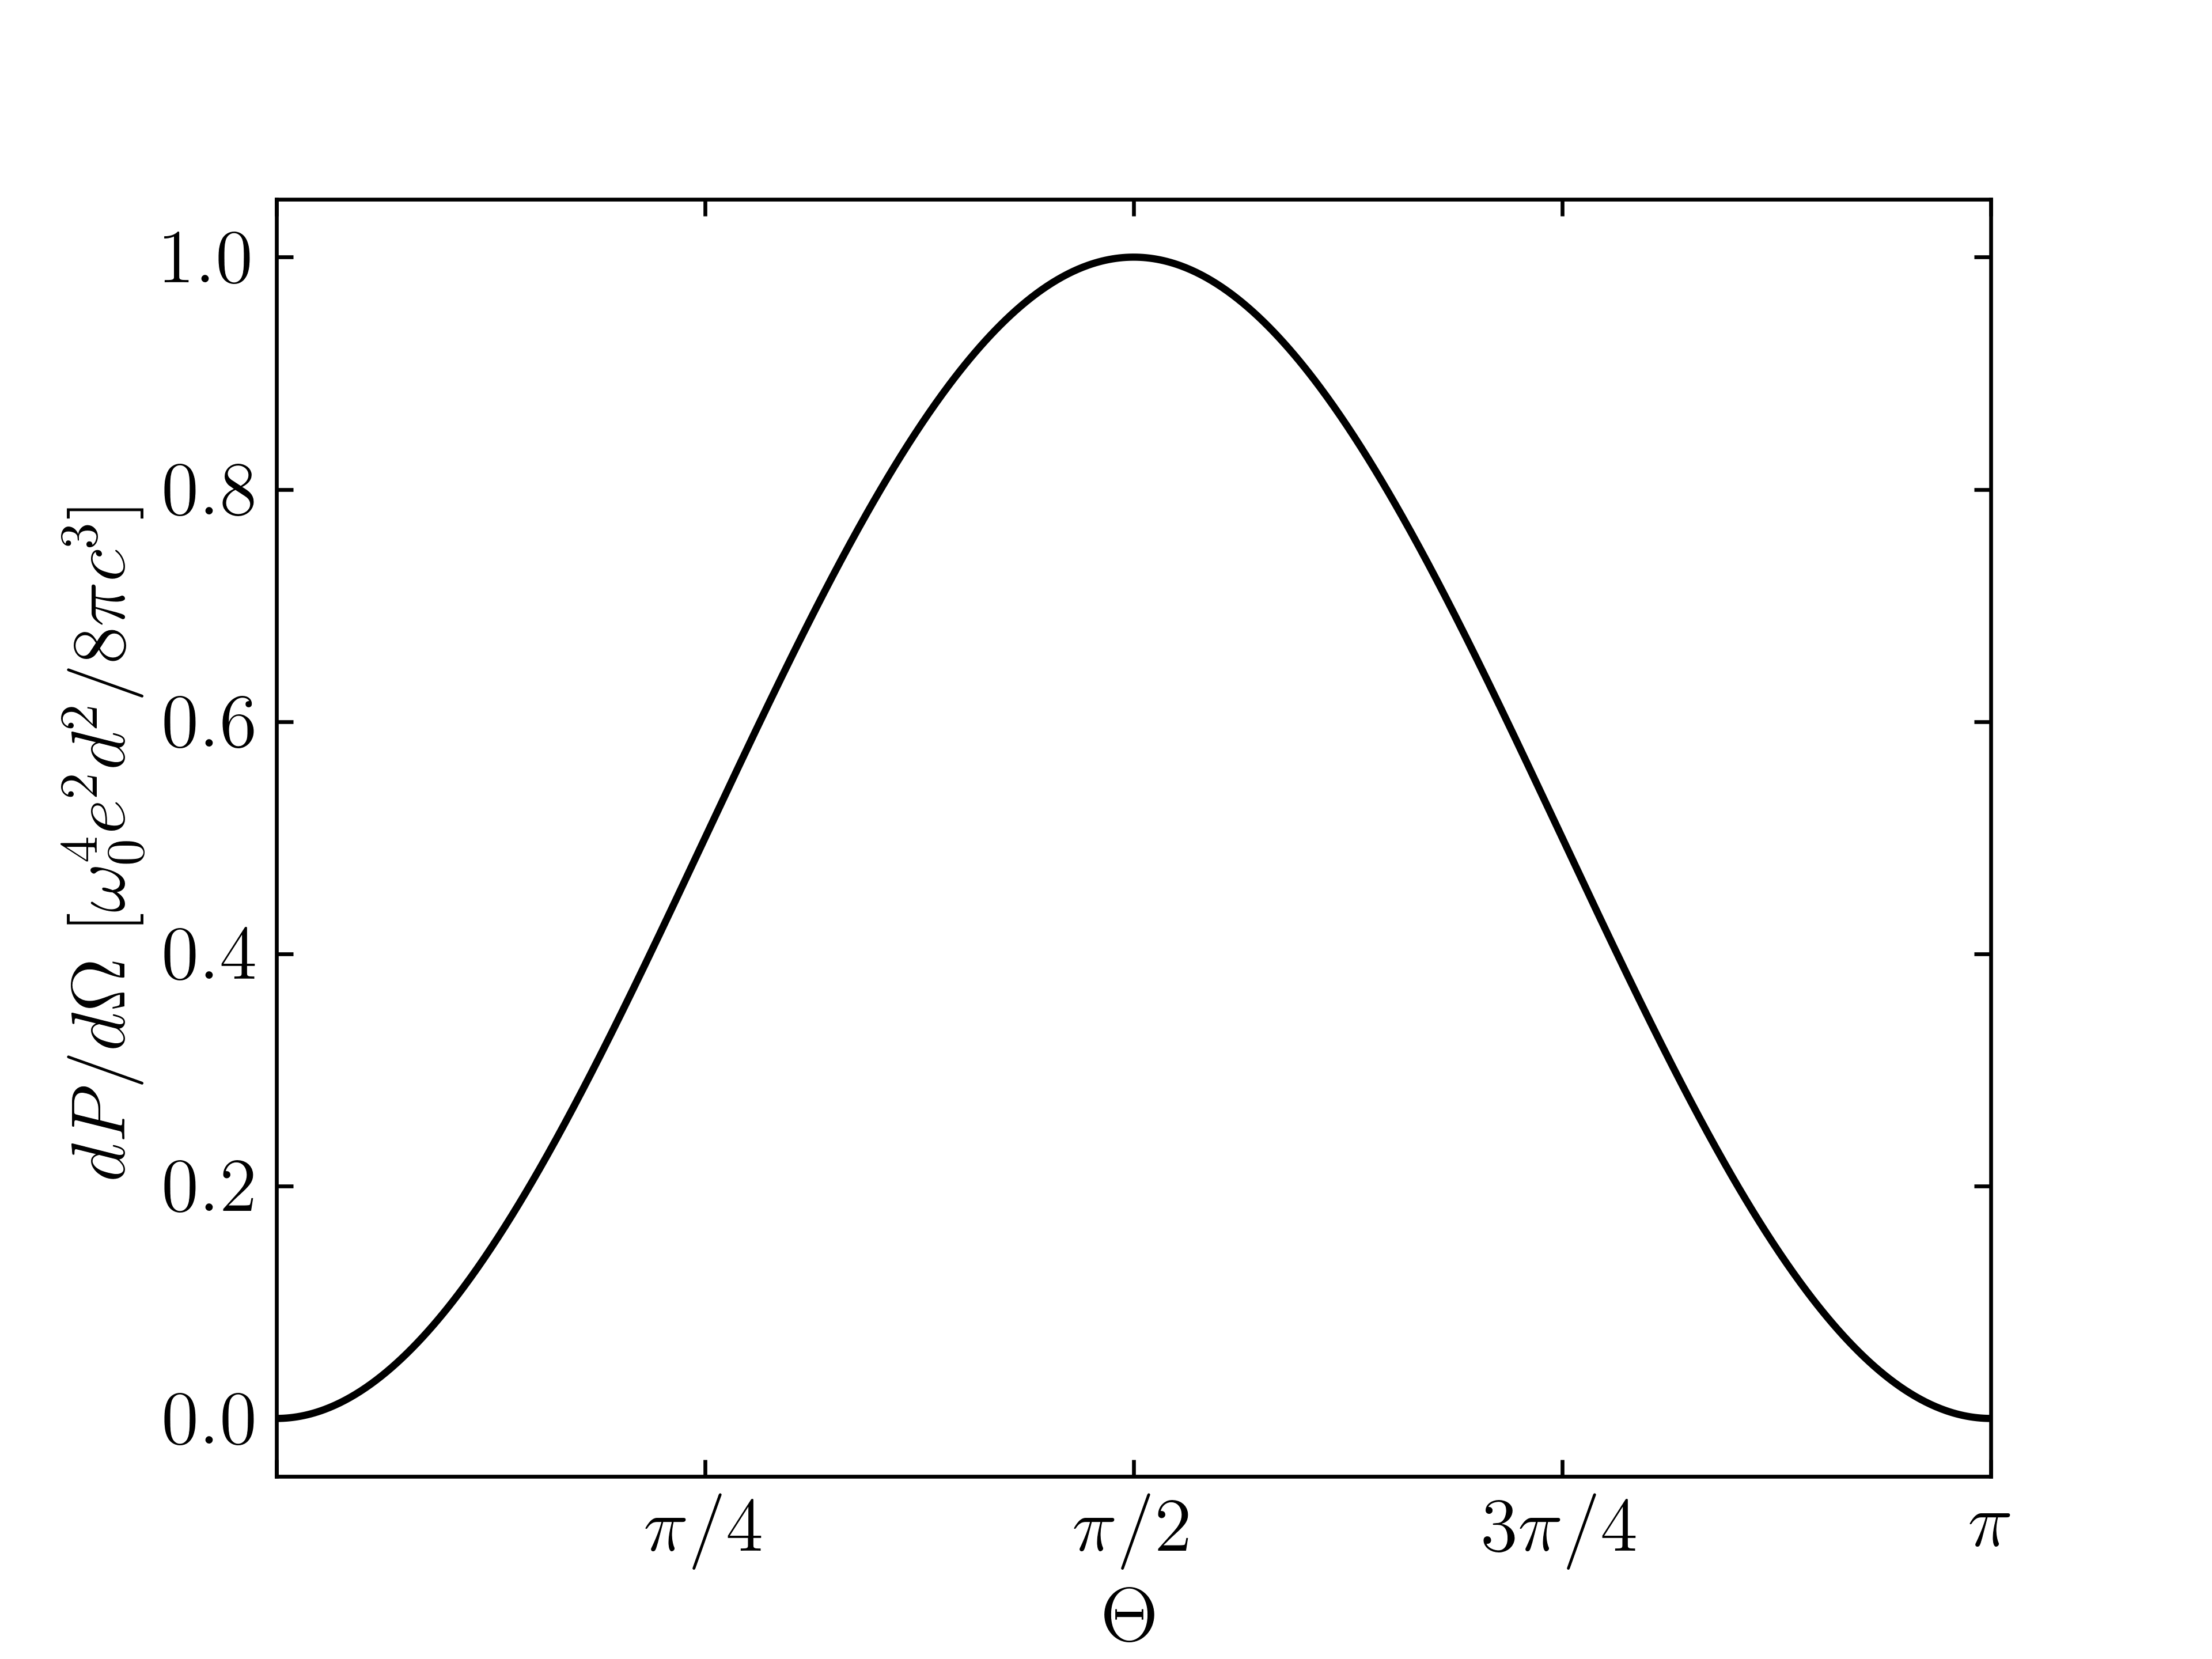
\includegraphics[width=0.8\textwidth]{p1a.png} 
\end{center}
We can also calculate the total radiated power
\begin{equation}
    P=\int \frac{dP}{d\Omega}d\Omega
    =\frac{e^2\omega_0^4d^2}{8\pi c^3}\int_{-1}^1 d(\cos\Theta)\sin^2\Theta
    \int_0^{2\pi}d\phi
    =\frac{\omega_0^4e^2d^2}{3c^3}.
\end{equation}

(b) The position of the charge can be written as
\begin{equation}
    \vb{r}_c=R(\cos\omega_0t\xhat+\sin\omega_0t\yhat).
    \Rightarrow \dot{\vb{r}}_c
    =\omega_0R(-\sin\omega_0t\xhat+\cos\omega_0t\yhat).
\end{equation}
Then, given that $\bm\omega=\omega_0\zhat$, the acceleration is
\begin{equation}\label{p1b:a}
    \vb{a}=\bm\omega\times\dot{\vb{r}}_c 
    =-\omega_0^2R(\cos\omega_0t\xhat+\sin\omega_0\yhat),
\end{equation}
which is, as expected from harmonic oscillation, $-\omega_0^2\vb{r}_c$. Also,
$\abs{\vb{a}}$ is constant since the charge is in circular orbit. It follows
from (14.21, Jackson) that
\begin{equation}
    \frac{dP}{d\Omega}=\frac{e^2}{4\pi c^3}\abs{\vb{a}}^2\sin^2\Theta
    =\frac{\omega_0^4e^2R^2}{4\pi c^3}\sin^2\Theta.
\end{equation}
The point of observation has the following coordinates
\begin{equation}\label{p1b:x}
    \vb{x}=r\qty(\sin\theta\cos\phi\xhat+\sin\theta\sin\phi\yhat+\cos\theta\zhat). 
\end{equation}
By definition, taking the dot product between \eqref{p1b:a} and \eqref{p1b:x} 
yields
\begin{equation}
    \cos\Theta=\frac{\vb{a}\vdot\vb{x}}{\abs{\vb{a}}\abs{\vb{x}}}
    =\sin\theta\cos(\omega_0t-\phi).
\end{equation}
Thus, the averaged radiation pattern is
\begin{align}\label{p1b:dP}
    \expval{\frac{dP}{d\Omega}}
    &=\frac{\omega_0^4e^2R^2}{4\pi
    c^3}\qty[1-\sin^2\theta\expval{\cos^2(\omega_0t-\phi)}]\notag\\
    &=\frac{\omega_0^4e^2R^2}{4\pi c^3}
    \qty[1-\frac12\sin^2\theta],
\end{align}
and the total radiated power is
\begin{equation}
    P=\frac{\omega_0^4e^2R^2}{2
    c^3}\int_{-1}^1d(\cos\theta)\qty[1-\frac12\sin^2\theta]
    =\frac{2\omega_0^4e^2R^2}{3c^3}.
\end{equation}
This agrees with (9.24, Jackson) for a dipole
\begin{equation}
    \vb{p}=eRe^{-i\omega t}\qty(\xhat+i\yhat). 
\end{equation}
A plot of \eqref{p1b:dP} is included below.
\begin{center}
    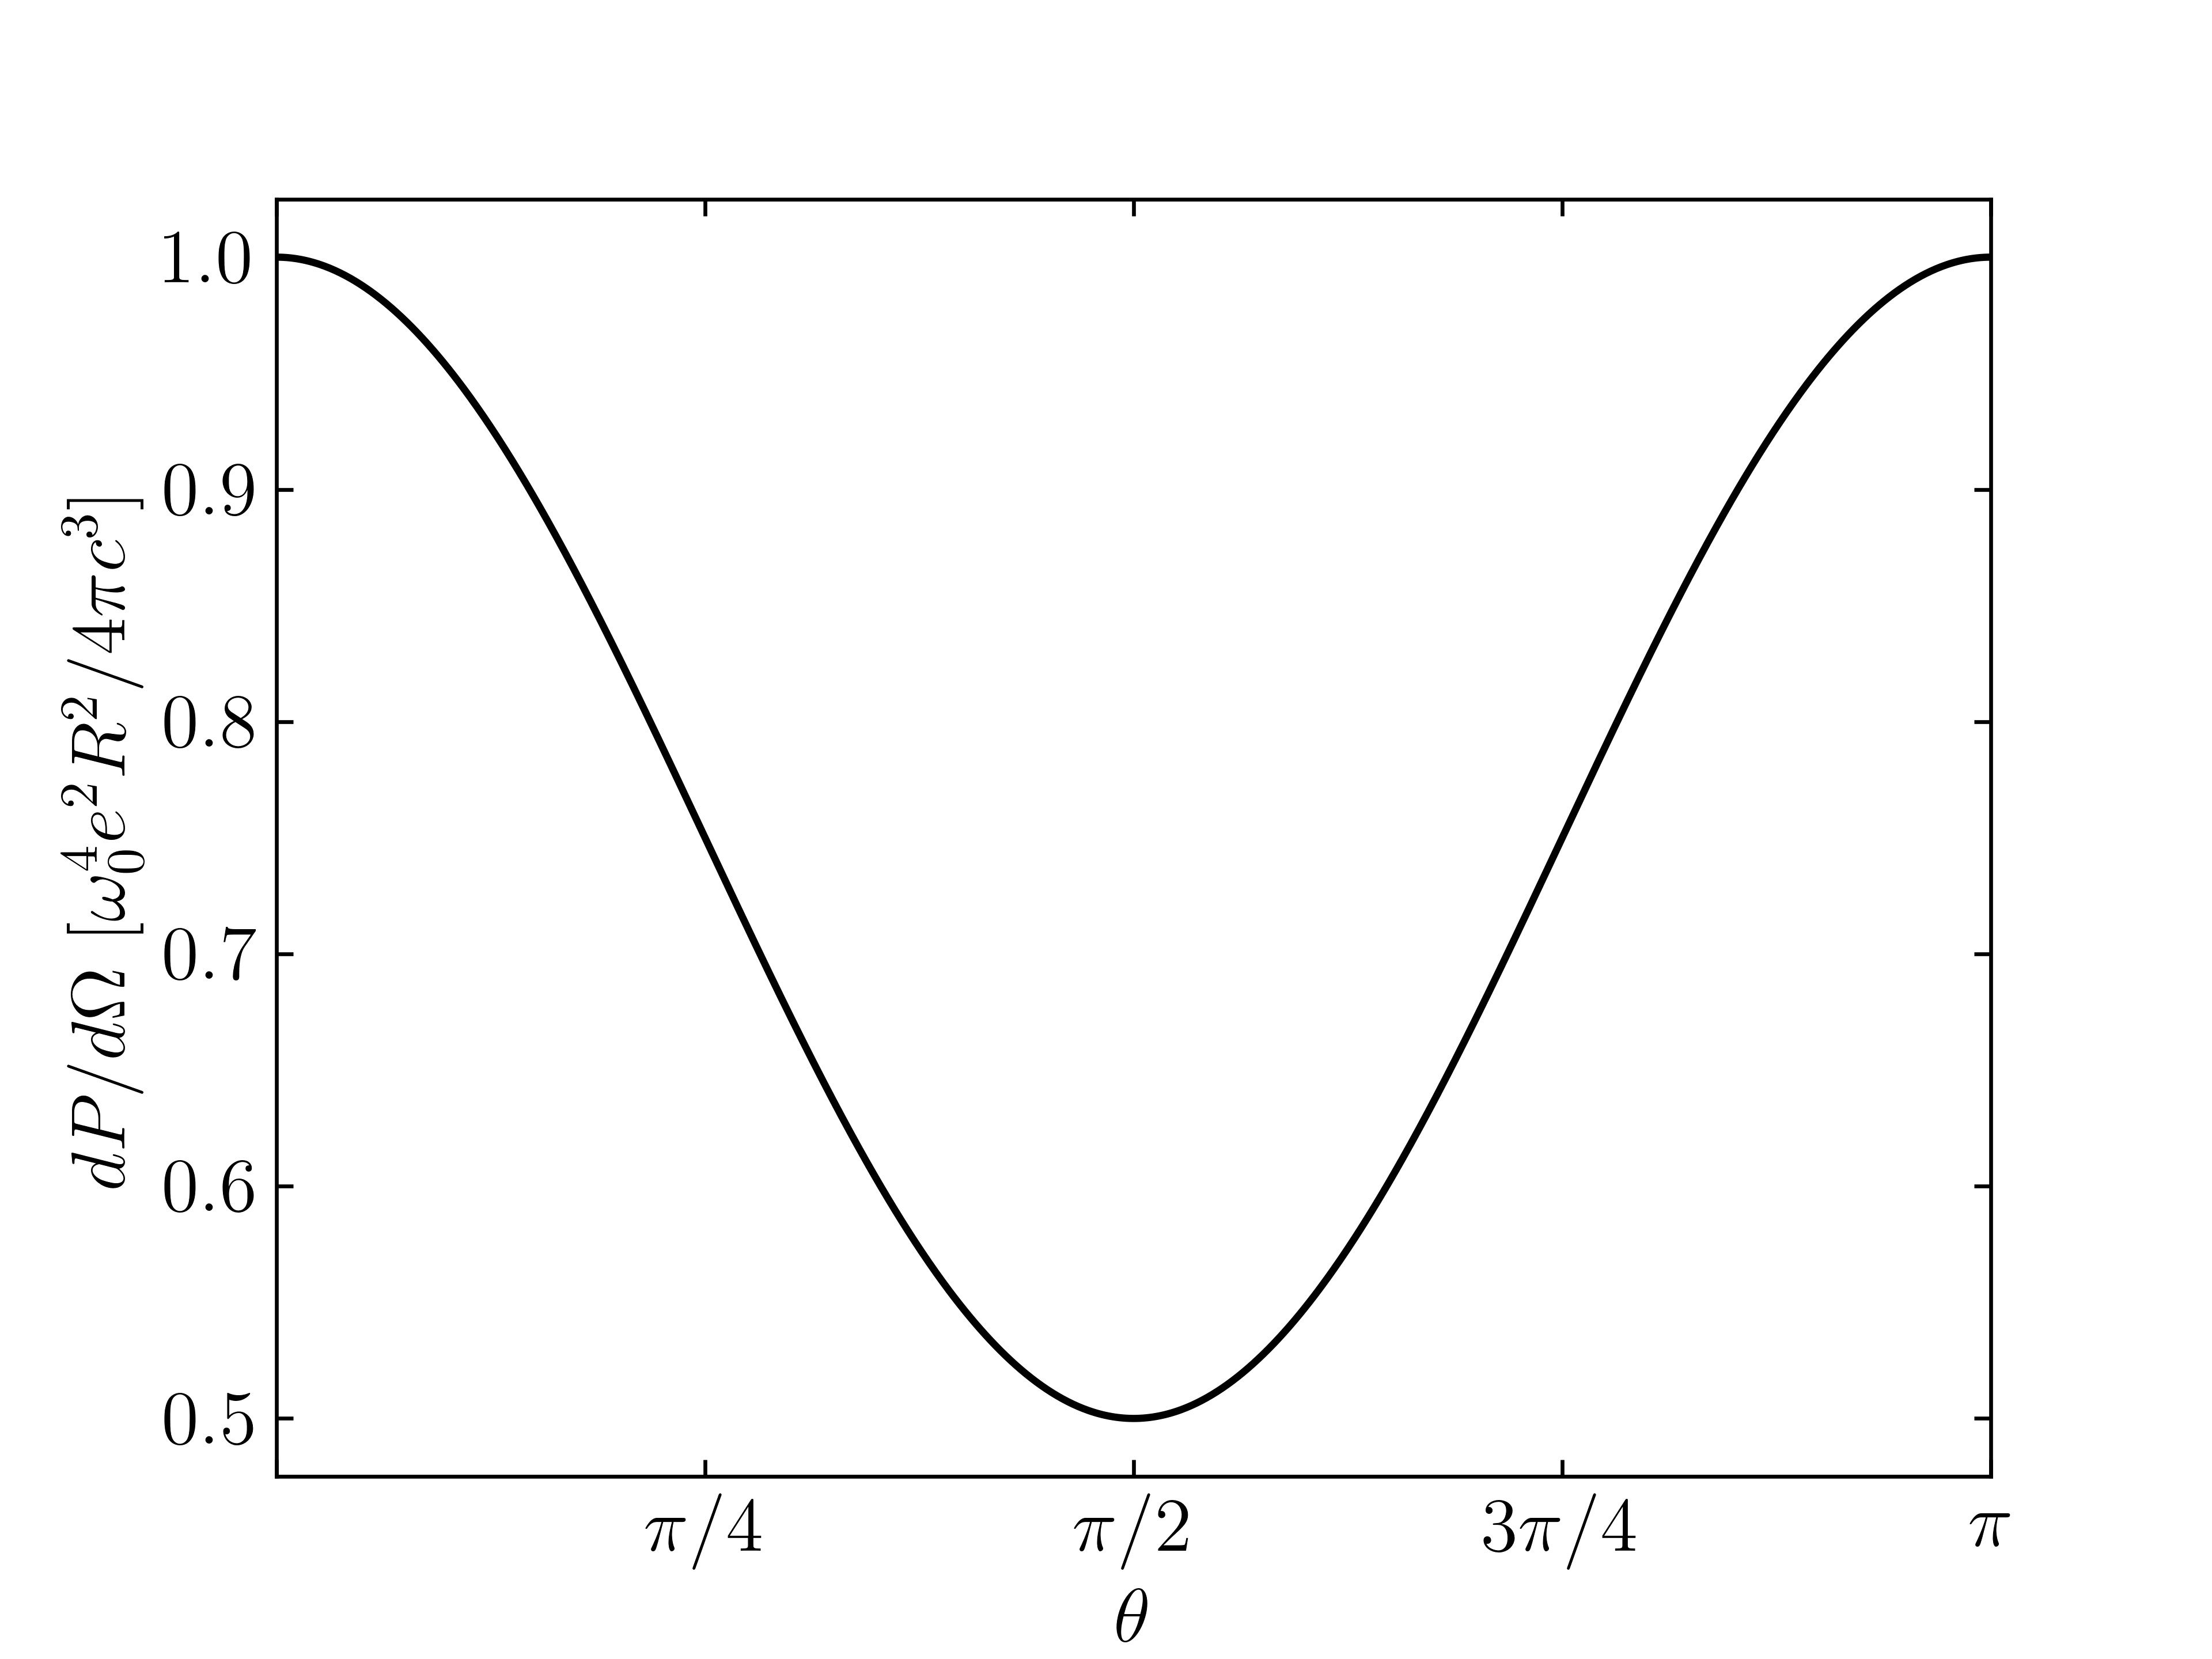
\includegraphics[width=0.8\textwidth]{p1b.png} 
\end{center}
\end{solution}
\end{problem}
\newpage
%%%%%%%%%%%%%%%%%%%%%%%%%%%%%%%%%%%%%%%%%%%%%%%%%%%%%%%%%%%%%%%%%%%%%%%%%%%%%%%    
%%%%%%%%%%%%%%%%%%%%%%%%%%%%%%%%%%%%%%%%%%%%%%%%%%%%%%%%%%%%%%%%%%%%%%%%%%%%%%%
\begin{problem}{2}[Radiation from motion in a magnetic field.]
A particle of mass $m$, charge $q$, moves in a plane perpendicular to a uniform,
static magnetic induction $B$.

(a) Calculate the total energy radiated per unit time, expressing it in terms of
the constants already defined and the ratio $\gamma$ of the particle's total
energy to its rest energy.

(b) If at time $t=0$ the particle has a total energy $E_0=\gamma_0mc^2$, show
that it will have energy $E=\gamma mc^2<E_0$ at a time $t$, where
\begin{equation}
    t\approx\frac{3m^3c^5}{2q^4B^2}\qty(\frac1\gamma-\frac1{\gamma_0}), 
\end{equation}
provided $\gamma\gg 1$.

(c) If the particle is initially nonrelativistic and has a \textit{kinetic}
energy $T_0$ at $t=0$, what is its kinetic energy at time $t$?
\begin{solution}
(a) The relativistic motion of a charged particle in a uniform magnetic field is
given in Jackson, Section 12.2
\begin{equation}
    \vb{v}=\omega R(\xhat-i\yhat)e^{-i\omega t},
\end{equation}
where $\omega=qB/\gamma mc$ is the relativistic gyrofrequency, $R$ is the
gyroradius, and we have set $v_\|=0$ since there is no acceleration in the
parallel direction. Since $\vb{v}$ is perpendicular to 
$\bm\omega$, we have
\begin{equation}
    \dot{\beta}=\abs{\bm\beta\times\bm\omega}=\beta\omega,\qquad\t{and}\qquad
    \abs{\bm\beta\times\dot{\bm\beta}}
    =\abs{\bm\beta\times(\bm\beta\times\bm\omega)}
    =-\beta^2\omega.
\end{equation}
From (14.26, Jackson), the total radiated power is
\begin{align}
    P
    &=\frac{2q^2}{3c}\gamma^6\qty[\dot\beta^2-(\bm\beta\times\dot{\bm\beta})^2]\notag\\
    &=\frac{2q^2}{3c}\gamma^6\qty[\beta^2\omega^2-\beta^4\omega^2]\notag\\
    &=\frac{2q^2}{3c}\gamma^4\beta^2\omega^2\notag\\
    &=\frac{2q^4B^2}{3m^2c^3}\beta^2\gamma^2\notag\\
    &=\frac{2q^4B^2}{3m^2c^3}(\gamma^2-1).
\end{align}

(b) The radiated power is $P=-(\partial E/\partial
t)=-mc^2(\partial\gamma/\partial t)$. Using the previous result, the time $t$ is
\begin{align}
    t=\int_0^tdt' 
    =-mc^2\int_{\gamma_0}^{\gamma}\frac{d\gamma}{P}
    =\frac{3m^3c^5}{2q^4B^2}\int_{\gamma_0}^\gamma\frac{d\gamma}{1-\gamma^2}.
\end{align}
But since $\gamma\gg 1$, we can ignore unity in the demoninator and write
\begin{equation}
    t\approx\frac{3m^3c^5}{2q^4B^2}\int_{\gamma_0}^\gamma\frac{d\gamma}{-\gamma^2}
    =\frac{3m^3c^5}{2q^4B^2}\qty(\frac1{\gamma}-\frac1{\gamma_0}).
\end{equation}

(c) In the non-relativistic regime, the gyrofrequency $\omega_0=qB/m$ is
constant, and we can utilize the result from Problem 1(b). Again assuming
$T_\|=0$ since the constant translation contributes nothing to the radiation, 
the kinetic energy is $T=(1/2)mv_\perp^2=(1/2)m\omega_0^2R^2$, and we can write 
the total radiated power as
\begin{equation}
    P=-\frac{\partial T}{\partial t}=\frac{4\omega_0^2e^2}{3mc^2}T\Rightarrow
    T(t)=T_0e^{-4\omega_0^2e^2 t/3mc^3}.
\end{equation}
So the kinetic energy is reduced exponentially with the rate
$\Gamma=4\omega_0^2e^2/3mc^3$.

\end{solution}
\end{problem}
\newpage
%%%%%%%%%%%%%%%%%%%%%%%%%%%%%%%%%%%%%%%%%%%%%%%%%%%%%%%%%%%%%%%%%%%%%%%%%%%%%%%
\end{document}
